% !TeX spellcheck = fr_FR
\chapter{Chapitre 1 : Données ATLAS}

Les données ATLAS, au cœur de cette étude, proviennent de la plateforme suisse Open Transport Data\citeref{ref:open_transport_data_swiss}. Cette ressource centralise les données des transports publics en Suisse, offrant une base précieuse pour l'analyse et le développement d'applications.\\

\medskip
\noindent\textbf{Reproductibilité.} Les figures et statistiques de ce chapitre ont été produites par des scripts reproductibles disponibles dans le répertoire \texttt{memoire/scripts\_used/} du dépôt Git du projet.


\section{Arrêts}

L'analyse des arrêts s'appuie sur le jeu de données \texttt{traffic-points-actual-date}\citeref{ref:traffic_points_actual_date}, qui recense les arrêts de transport public en Suisse en fournissant des informations détaillées sur leur localisation et leurs caractéristiques. Ces points peuvent être visualisés sur une carte interactive via l’application web https://atlas.app.sbb.ch/\citeref{ref:atlas_app_sbb}.

Nous nous concentrons ici sur deux colonnes principales : le \texttt{number} et la \texttt{designation} de chaque arrêt.

Le numéro d’un arrêt correspond à la référence UIC (Union Internationale des Chemins de fer), un standard international pour l'identification des lieux de transport public. Les deux premiers chiffres représentent le code du pays ; la Suisse, par exemple, utilise le code 85\citeref{ref:wikipedia_uic_codes}. Ainsi, un numéro UIC comme \texttt{ 8502034} désigne un arrêt spécifique du réseau suisse.

La colonne \texttt{designation} fait référence à une identification locale : une valeur de \texttt{3} peut, par exemple, indiquer que l’arrêt correspond à la plateforme 3 d’une gare.

Enfin, les données incluent également des informations sur l’opérateur responsable de chaque arrêt, un élément utile pour établir des correspondances avec d’autres jeux de données.

Le jeu de données distingue deux types de \texttt{trafficPointElementType} : \texttt{BOARDING\_AREA} et \texttt{BOARDING\_PLATFORM}. Notre analyse se limite aux \texttt{BOARDING\_PLATFORM}, car les \texttt{BOARDING\_AREA} ne disposent pas de coordonnées géographiques. Pour extraire ces informations, nous avons développé un script Python, \texttt{get\_atlas\_data.py}. Extrait simplifié du chargement/filtrage:

\begin{codebox}[language=Python]{Extrait — \texttt{get\_atlas\_stops}}
def get_atlas_stops(output_path, download_url):
    response = requests.get(download_url)
    response.raise_for_status()
    with zipfile.ZipFile(io.BytesIO(response.content)) as z:
        csv_filename = z.namelist()[0]
        with z.open(csv_filename) as f:
            df = pd.read_csv(f, sep=';')
            # Suisse (UIC pays = 85)
            df = df[df['uicCountryCode'] == 85]
            # Filtre frontière CH: inclusion dans le polygone suisse (WGS84)
            df = filter_points_in_switzerland(df, lat_col='wgs84North', lon_col='wgs84East')
            # Comptage des quais
            boarding_platforms = df[df['trafficPointElementType'] == 'BOARDING_PLATFORM']
            df.to_csv(output_path, sep=';', index=False)
\end{codebox}


\paragraph{Statistiques ATLAS.} Sur l'instantané analysé (après filtre UIC=85 et frontière CH par polygone) :
\begin{itemize}
  \item \textbf{Lignes avec coordonnées (dans la frontière CH)}: \textit{55\,571}.
  \item \textbf{\texttt{BOARDING\_PLATFORM}}: \textit{54\,882}.
  \item \textbf{UIC distincts (\texttt{number})}: \textit{26\,750}.
  \item \textbf{\texttt{designation} non vides}: \textit{12\,051} (\textit{538} valeurs distinctes).
  \item \textbf{\texttt{designation} manquantes}: \textit{43\,520}, dont \textit{4\,365} cas où l'unique entrée du \texttt{number} est sans désignation.
  \item \textbf{Entrées identifiables par (\texttt{number}, \texttt{designation}) seul}: \textit{10\,514}.
  \item \textbf{Total identifiables par \texttt{number} + (\texttt{designation} ou unicité du \texttt{number})}: \textit{15\,854}.
\end{itemize}

\begin{figure}[H]
  \centering
  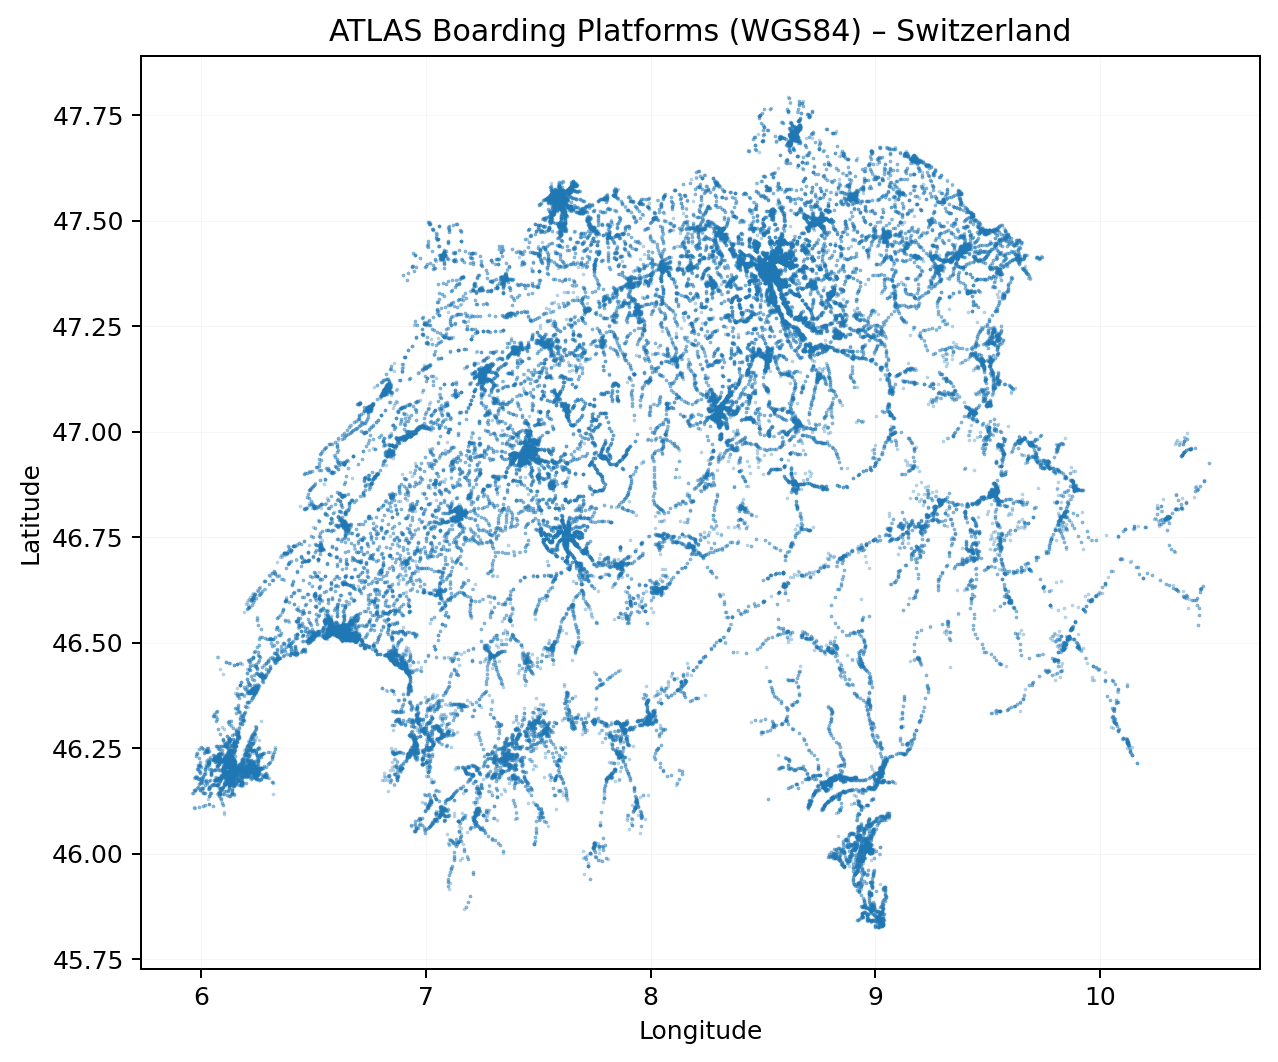
\includegraphics[width=.76\linewidth]{figures/plots/atlas_points_switzerland.png}
  \caption[ATLAS: distribution nationale]{ATLAS: distribution nationale (WGS84).}
  \label{fig:atlas_ch_points}
\end{figure}

\begin{figure}[H]
  \centering
  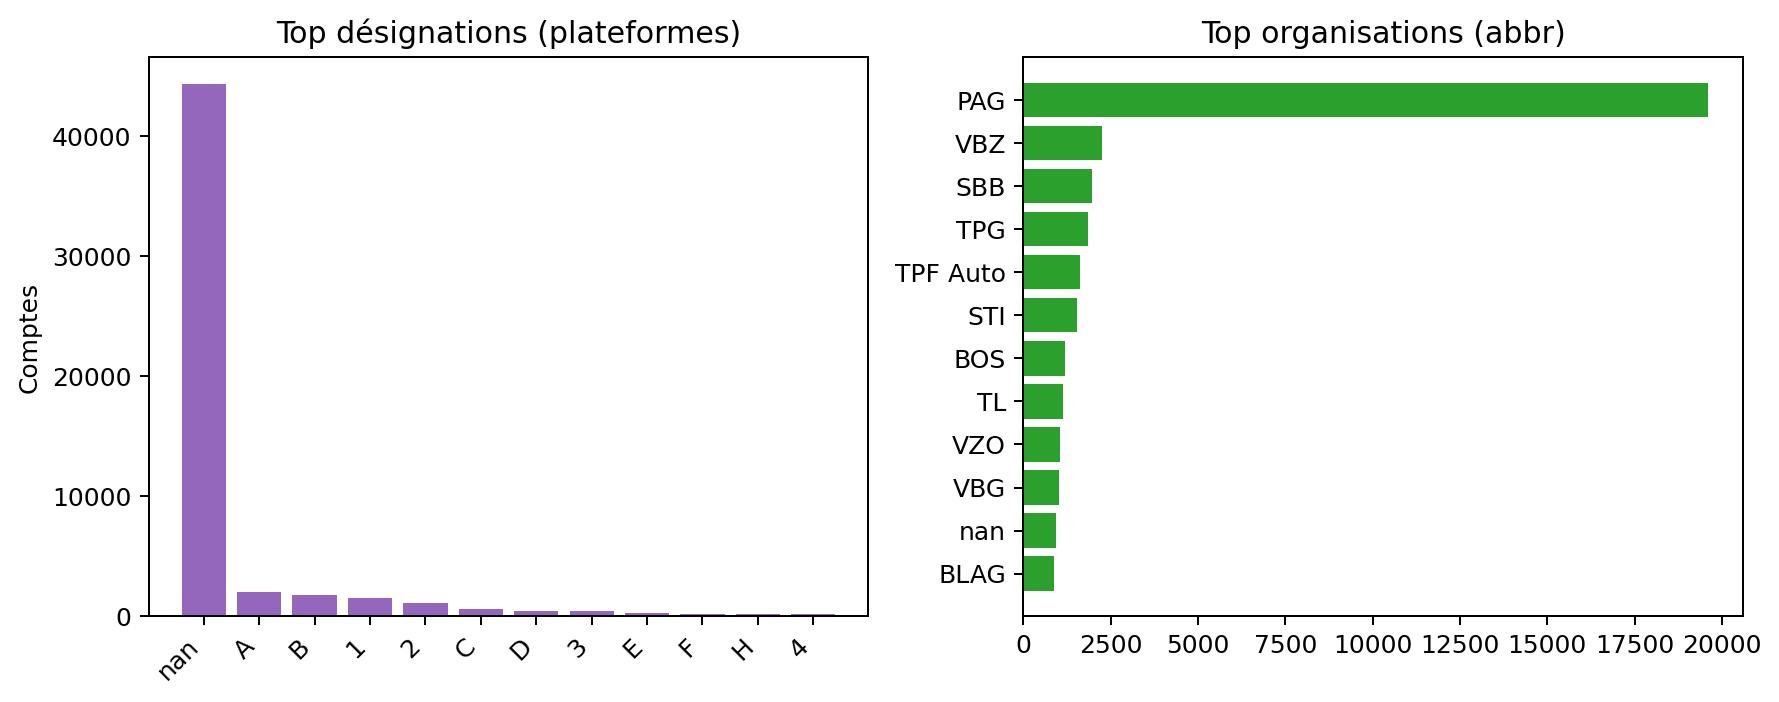
\includegraphics[width=.85\linewidth]{figures/plots/atlas_designation_operators.png}
  \caption[Désignations et opérateurs ATLAS]{À gauche: désignations de plateforme les plus fréquentes (hors valeurs manquantes). À droite: principales organisations (abrégés) déclarées.}
  \label{fig:atlas_distribs}
\end{figure}

\noindent\textit{Remarque.} Les très nombreuses valeurs manquantes pour \texttt{designation} sont exclues du classement afin d'éviter un effet disproportionné. Comme indiqué plus haut, \(43\,520\) entrées n'ont pas de \texttt{designation}.

Concernant les coordonnées, le fichier fournit deux systèmes : le système de référence suisse LV95 et le système de référence global WGS84. Étant donné que les données d'OpenStreetMap (OSM) utilisent les coordonnées WGS84, nous nous concentrerons sur cet ensemble de coordonnées.

\section{GTFS}

Le General Transit Feed Specification (GTFS) est un format d'échange numérique initié par Google pour standardiser les horaires des transports publics et leurs informations géographiques, telles que la localisation des arrêts. En Suisse, ces données sont publiées sur la plateforme OpenTransportDataSuisse\citeref{ref:gtfs_cookbook}. Elles servent à développer des applications pratiques, comme les outils de consultation d'horaires ou de planification de trajets.

Bien que notre projet se focalise actuellement sur la synchronisation des arrêts, les données GTFS relatives aux trajets retiennent également notre attention. Elles pourraient faciliter la correspondance entre les arrêts ATLAS et ceux d’OpenStreetMap, en exploitant les informations sur les itinéraires présentes dans les deux ensembles de données. Parmi les  fichiers GTFS, quatre retiennent notre attention : \texttt{stops.txt}, \texttt{stop\_times.txt}, \texttt{routes.txt} et \texttt{trips.txt}.

\subsection{Description des fichiers}

Les fichiers GTFS suivants sont cruciaux pour notre analyse :

\begin{itemize}
    \item \textbf{\texttt{stops.txt}} : Ce fichier répertorie les arrêts avec leurs coordonnées géographiques et d’autres attributs. 
    Un extrait est présenté dans le tableau \ref{tab:stops}.
    \item \textbf{\texttt{routes.txt}} : Il décrit les lignes de transport, avec des informations comme le nom court, le nom long, et le type de transport. 
    Voir le tableau \ref{tab:routes}.
    \item \textbf{\texttt{trips.txt}} : Ce fichier associe les trajets aux lignes et aux services.
    Un exemple est donné dans le tableau \ref{tab:trips}.
    \item \textbf{\texttt{stop\_times.txt}} : Il contient les horaires d’arrivée et de départ pour chaque arrêt d’un trajet.
    Voir le tableau \ref{tab:stop_times}.
    \begin{table}[H]
    \caption{Extrait du fichier \texttt{stops.txt}}
    \label{tab:stops}
    \centering
    \begin{tabular}{l l r r l l}
    \toprule
    stop\_id & stop\_name & stop\_lat & stop\_lon  & parent\_station \\
    \midrule
    1101064 & Malpensa Aeroporto, terminal 1 & 45.6272 & 8.7111 & \\
    8000339 & Weissenhorn Eschach & 48.3010 & 10.1351  & \\
    8000709:0:2 & Neckarsulm Mitte & 49.1935 & 9.2229  & \\
    8000778 & Asselheim (D) & 49.5762 & 8.1616  & \\
    8000781 & Grünstadt-Nord & 49.5734 & 8.1708 & \\
    8000988 & Witzighausen & 48.3174 & 10.0978 & \\
    8002015 & Nördlingen & 48.8508 & 10.4979 & 8002015P \\
    8002015:0:4 & Nördlingen & 48.8509 & 10.4979 & 8002015P \\
    \bottomrule
    \end{tabular}
    \end{table}

    \begin{table}[H]
    \caption{Extrait du fichier \texttt{routes.txt}}
    \label{tab:routes}
    \centering
    \begin{tabular}{l l l l l l}
    \toprule
    route\_id & agency\_id & route\_short\_name & route\_desc & route\_type \\
    \midrule
    91-10-A-j22-1 & 37 & 10 & T & 900 \\
    91-10-B-j22-1 & 78 & S10 & S & 109 \\
    91-10-C-j22-1 & 11 & S10 & S & 109 \\
    91-10-E-j22-1 & 65 & S10 & S & 109 \\
    91-10-F-j22-1 & 11 & RE10 & RE & 106 \\
    91-10-G-j22-1 & 11 & SN10 & SN & 109 \\
    91-10-j22-1 & 3849 & 10 & T & 900 \\
    91-10-Y-j22-1 & 82 & IR & IR & 103 \\
    \bottomrule
    \end{tabular}
    \end{table}

    \begin{table}[H]
    \caption{Extrait du fichier \texttt{trips.txt}}
    \label{tab:trips}
    \centering
    \begin{tabular}{l l l l l l l l l}
    \toprule
    route\_id & trip\_id & trip\_short\_name & direction\_id  \\
    \midrule
    91-8-H-j25-1  & 994.TA.91-8-H-j25-1.59.R  & 6278 & 1 \\
    91-8-H-j25-1  & 995.TA.91-8-H-j25-1.59.R  & 2978 & 1 \\
    91-8-H-j25-1  & 996.TA.91-8-H-j25-1.59.R & 2787 & 1 \\
    91-8-H-j25-1  & 997.TA.91-8-H-j25-1.59.R  & 4879 & 1 \\
    91-8-H-j25-1  & 998.TA.91-8-H-j25-1.59.R  & 10407 & 1 \\
    91-8-H-j25-1  & 999.TA.91-8-H-j25-1.59.R  & & 1 & \\
    \bottomrule
    \end{tabular}
    \end{table}

    \begin{table}[H]
    \caption{Extrait du fichier \texttt{stop\_times.txt}}
    \label{tab:stop_times}
    \centering
    \begin{tabular}{l l l l r l l}
    \toprule
    trip\_id & arrival\_time & departure\_time & stop\_id & stop\_sequence \\
    \midrule
    1.TA.1-9-j17-1.1.H & 05:25:00 & 05:25:00 & 8502034:0:2 & 1 \\
    1.TA.1-9-j17-1.1.H & 05:28:00 & 05:29:00 & 8502033:0:2 & 2 \\
    1.TA.1-9-j17-1.1.H & 05:33:00 & 05:33:00 & 8502032:0:1 & 3 \\
    1.TA.1-9-j17-1.1.H & 05:36:00 & 05:36:00 & 8502031:0:1 & 4 \\
    1.TA.1-9-j17-1.1.H & 05:42:00 & 05:42:00 & 8502030:0:2 & 5 \\
    1.TA.1-9-j17-1.1.H & 05:50:00 & 05:50:00 & 8502119:0:7 & 6 \\
    2.TA.1-9-j17-1.2.H & 05:53:00 & 05:53:00 & 8502034:0:1 & 1 \\
    2.TA.1-9-j17-1.2.H & 05:57:00 & 05:58:00 & 8502033:0:2 & 2 \\
    \bottomrule
    \end{tabular}
    \end{table}
\end{itemize}


\subsection{Clés d’identification, normalisation et jointure}

Dans le script \texttt{get\_atlas\_data.py}, nous construisons un jeu de données intégré qui associe chaque arrêt aux couples \texttt{(route\_id, direction\_id)} desservis et aux noms de lignes, puis relions ces arrêts aux SLOIDs ATLAS. La jointure exploite \texttt{stop\_times.txt} pour relier les arrêts aux trajets via \texttt{trip\_id}, puis \texttt{trips.txt} et \texttt{routes.txt} pour relier ces trajets aux lignes via \texttt{route\_id}. Nous dédupliquons ensuite les paires route–direction par arrêt et ajoutons le nom de ligne.

\medskip
\noindent\textbf{Clé de correspondance stop\_id GTFS \(\to\) SLOID ATLAS.} Nous associons \texttt{stop\_id} (GTFS) aux SLOIDs ATLAS via \texttt{number} (UIC) et \texttt{designation} (référence locale de quai), avec normalisation minimale. Les règles, \emph{telles qu'implémentées dans le code}, sont les suivantes:
\begin{itemize}
  \item \textbf{Structure de \texttt{stop\_id}}: \texttt{uic\_number:0:local\_ref}. Exemple: \texttt{8516155:0:1}.
  \item \textbf{Strict}: associer si \(\texttt{uic\_number} = \texttt{number}\) et \(\texttt{normalized\_local\_ref} = \texttt{designation}\).
  \item \textbf{Fallback 1} (si non associé strictement): si le \texttt{number} côté ATLAS n’a qu’une seule ligne, utiliser son \texttt{sloid}.
  \item \textbf{Fallback 2} (sinon): si la dernière composante du \texttt{sloid} (après les \texttt{:}) est égale à \texttt{normalized\_local\_ref}, utiliser ce \texttt{sloid}.
  \item \textbf{Normalisation}: les références locales \enquote{10000/10001} sont ramenées à \enquote{1/2} lorsqu’elles codent des côtés/plates-formes.
\end{itemize}

La mise en correspondance entre la colonne \texttt{stop\_id} du fichier \texttt{stops.txt} (GTFS) et l’identifiant \texttt{sloid} d’ATLAS présente des défis importants. Premièrement, il n’existe pas de lien direct entre ces deux identifiants. Deuxièmement, les coordonnées géographiques des arrêts diffèrent entre les deux ensembles de données.

\textbf{Exemple 1 : "Lancy-Pont-Rouge":}
\newline
Considérons la gare "Lancy-Pont-Rouge", opérée par les CFF. Dans le fichier \texttt{stops.txt} de GTFS, les données sont les suivantes :

\begin{table}[H]
\caption{Extrait de \texttt{stops.txt} pour "Lancy-Pont-Rouge"}
\label{tab:stops_lancy_2}
\centering
\begin{tabular}{l l r r l l}
\toprule
\texttt{stop\_id} & \texttt{stop\_name} & \texttt{stop\_lat} & \texttt{stop\_lon} & \texttt{parent\_station} \\
\midrule
8516155:0:1 & Lancy-Pont-Rouge & 46.18596197 & 6.12483039 & Parent8516155 \\
8516155:0:2 & Lancy-Pont-Rouge & 46.18595575 & 6.12495615 & Parent8516155 \\
\bottomrule
\end{tabular}
\end{table}

Dans le fichier \texttt{traffic-points-actual-data}, on trouve :

\begin{table}[H]
\caption{Extrait de \texttt{traffic-points-actual-data} pour "Lancy-Pont-Rouge"}
\label{tab:traffic_lancy_2}
\centering
\begin{tabular}{l l l l r r l}
\toprule
\texttt{sloid} & \texttt{number} & \texttt{des.} & \texttt{wgs84East} & \texttt{wgs84North} & \texttt{designationOfficial} \\
\midrule
...:16155:1:1 & 8516155 & 1  & 6.12483137 & 46.18596333 & Lancy-Pont-Rouge \\
...:16155:1:2 & 8516155 & 2  & 6.12495213 & 46.18595284 & Lancy-Pont-Rouge \\
\bottomrule
\end{tabular}
\end{table}

Ici, le format de \texttt{stop\_id} dans GTFS est \texttt{uic\_number:0:local\_ref}, où \texttt{uic\_number} correspond à la colonne \texttt{number} dans ATLAS (8516155), et \texttt{local\_ref} à \texttt{designation} (1 ou 2). Cela permet une correspondance, bien que les coordonnées géographiques divergent légèrement.

\textbf{Exemple 2 : "Lausanne Bourdonnette":}
\newline
Prenons un deuxième exemple avec "Lausanne Bourdonnette". Dans \texttt{stops.txt} :
\begin{table}[H]
\caption{Extrait de \texttt{stops.txt} pour "Lausanne Bourdonnette"}
\label{tab:stops_bourdonnette_2}
\centering
\begin{tabular}{l l r r}
\toprule
\texttt{stop\_id} & \texttt{stop\_name} & \texttt{stop\_lat} & \texttt{stop\_lon} \\
\midrule
8501210:0:10000 & Lausanne, Bourdonnette & 46.52342565 & 6.59074161 \\
8501210:0:10001 & Lausanne, Bourdonnette & 46.52329585 & 6.58987025 \\
8501210:0:A & Lausanne, Bourdonnette & 46.52326494 & 6.58980736 \\
8501210:0:B & Lausanne, Bourdonnette & 46.52318459 & 6.58978940 \\
8501210:0:C & Lausanne, Bourdonnette & 46.52272720 & 6.58913363 \\
8501210:0:D & Lausanne, Bourdonnette & 46.52338238 & 6.59138840 \\
\bottomrule
\end{tabular}
\end{table}

Et dans \texttt{traffic-points-actual-data} :

\begin{table}[H]
\caption{Extrait de \texttt{traffic-points-actual-data} pour "Lausanne Bourdonnette"}
\label{tab:traffic_bourdonnette_2}
\centering
\begin{tabular}{l l l l r r l}
\toprule
\texttt{sloid} & \texttt{number} & \texttt{des.
}  & \texttt{wgs84East} & \texttt{wgs84North} & \texttt{designationOfficial} \\
\midrule
...:1210:0:1600 & 8501210 &  & 6.59074107 & 46.52342597 & Lausanne, Bourdonnette \\
...:1210:0:1610 & 8501210 &  & 6.58986994 & 46.52329351 & Lausanne, Bourdonnette \\
...:1210:0:1616 & 8501210 & B & 6.58979344 & 46.52318499 & Lausanne, Bourdonnette \\
...:1210:0:2597 & 8501210 & D & 6.59138793 & 46.52338108 & Lausanne, Bourdonnette \\
...:1210:0:2542 & 8501210 & C & 6.58913042 & 46.52272550 & Lausanne, Bourdonnette \\
\bottomrule
\end{tabular}
\end{table}

Dans ce cas, les désignations dans GTFS incluent "A", "B", "C", "D", ainsi que des références numériques comme "10000" et "10001", mais dans ATLAS,  "A" n’a pas d’équivalent direct, et les références numériques ne sont pas assignées (lignes avec \texttt{designation} vide). Les coordonnées géographiques diffèrent également.

\subsection{Résultats}
Nous obtenons un jeu intégré listant, par \texttt{sloid}, les couples \texttt{(route\_id, direction\_id)}. Sur notre jeu:
\begin{itemize}
  \item \textbf{SLOIDs couverts par GTFS}: \textit{34\,415}.
  \item \textbf{Médiane des lignes par SLOID (GTFS)}: \textit{2}.
\end{itemize}

\begin{figure}[h]
  \centering
  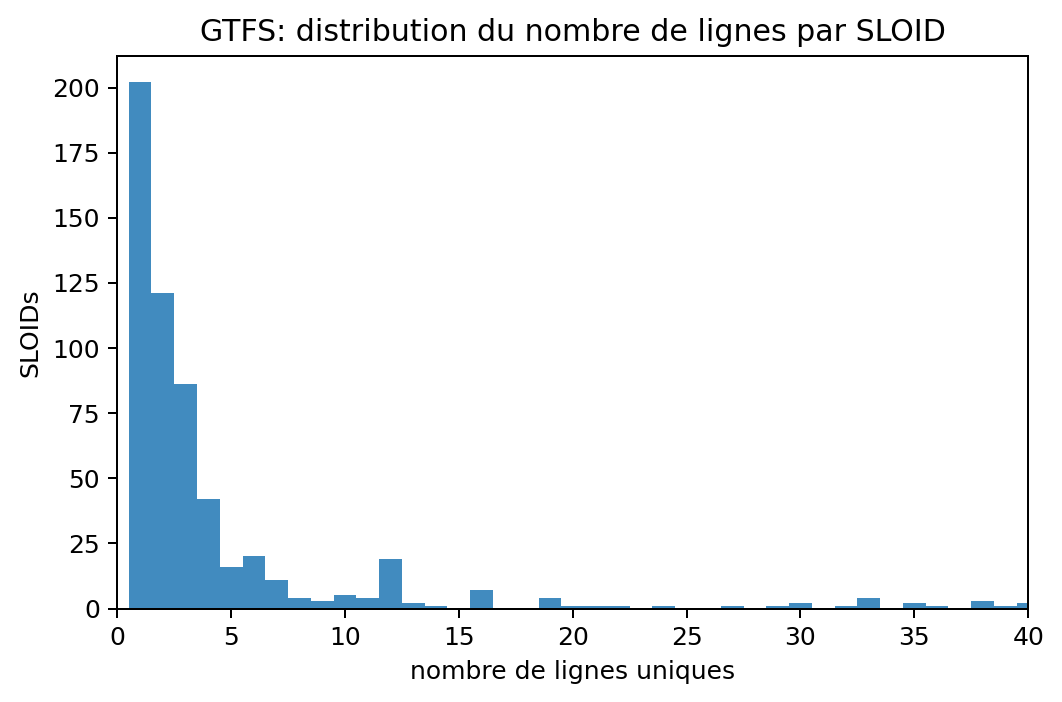
\includegraphics[width=.7\linewidth]{figures/plots/gtfs_routes_per_sloid.png}
  \caption[GTFS: lignes par SLOID]{GTFS: distribution du nombre de lignes par SLOID.}
  \label{fig:gtfs_lines_per_sloid}
\end{figure}

\begin{figure}[h]
  \centering
  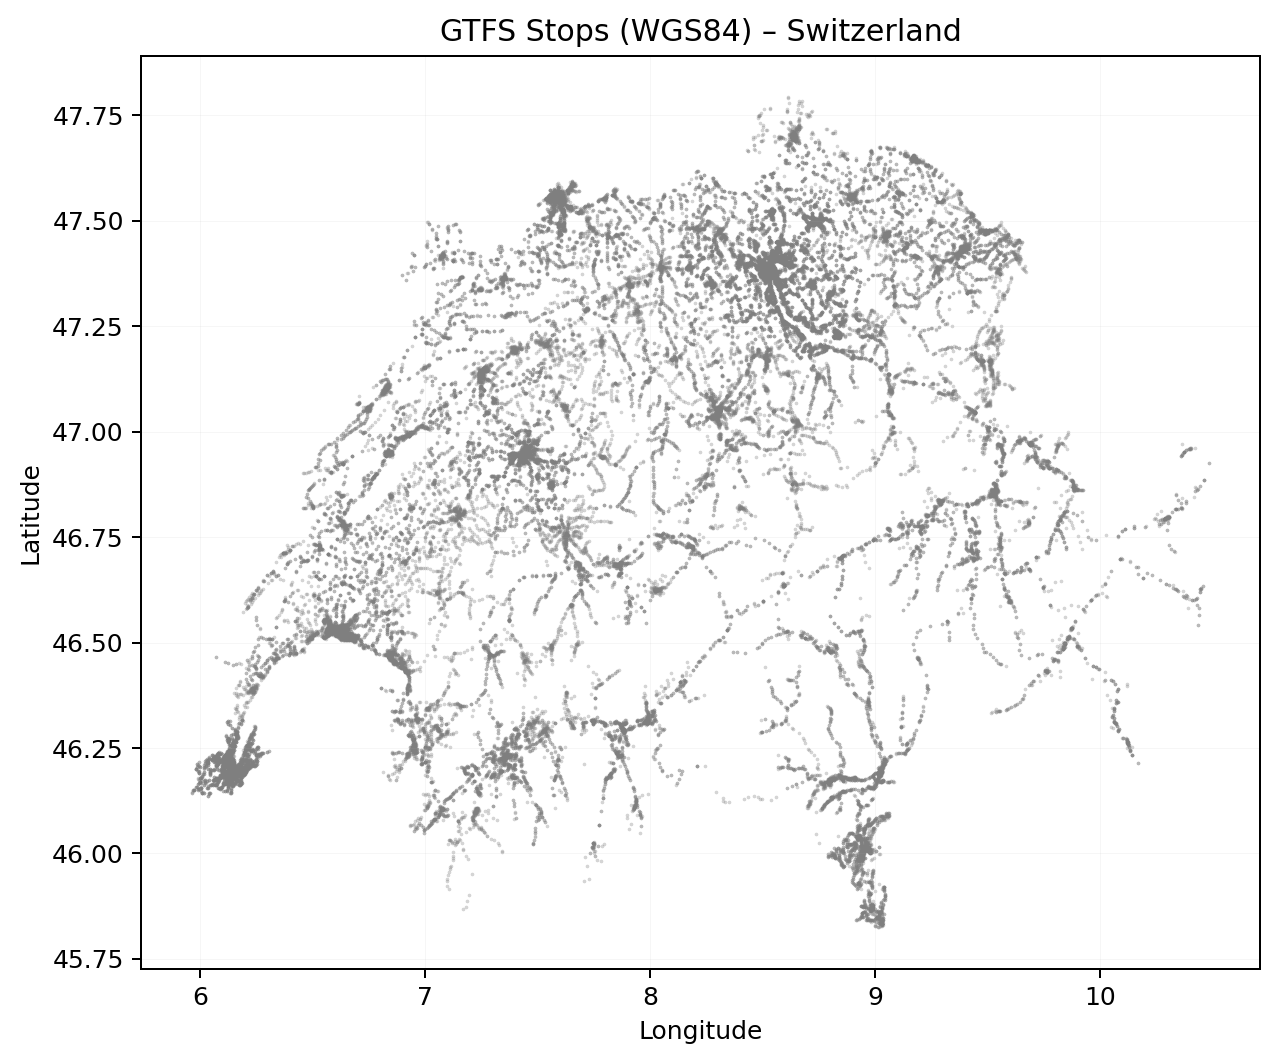
\includegraphics[width=.76\linewidth]{figures/plots/gtfs_points_switzerland.png}
  \caption[Arrêts GTFS (Suisse)]{Arrêts GTFS (Suisse, à l'intérieur de la frontière): \(47\,567\) arrêts détectés.}
  \label{fig:gtfs_ch_points}
\end{figure}




\vspace{.2em}

\section{HRDF}
Le format \textit{HAFAS Raw Data Format} (HRDF) structure des jeux de données d'horaires exhaustifs. Deux fichiers sont clés: \texttt{BHFART} (SLOIDs gare/quai) et \texttt{GLEISE\_WGS/LV95} (infrastructure et coordonnées de quai).

\noindent\textit{Référence.} Une description synthétique et à jour du format HRDF est disponible dans le Cookbook de la plateforme Open Transport Data Switzerland\footnote{\url{https://opentransportdata.swiss/en/cookbook/timetable-cookbook/hafas-rohdaten-format-hrdf/}}.

\subsection{Comment nous le lisons}
L'extraction des informations de direction à partir des données HRDF est un processus en plusieurs étapes, orchestré par le script \texttt{get\_atlas\_data.py}. Notre approche est conçue pour être efficace, en ne traitant que les données pertinentes pour les arrêts ATLAS (SLOIDs) que nous cherchons à enrichir.

\begin{enumerate}
    \item \textbf{Identification des voyages par quai (\texttt{GLEISE\_LV95}).}
    La première étape consiste à identifier les voyages (trajets) qui desservent chaque quai d'intérêt. Pour ce faire, nous parcourons le fichier \texttt{GLEISE\_LV95} en deux passes :
    \begin{itemize}
        \item D'abord, nous établissons une correspondance entre chaque \texttt{sloid} de quai et son couple identifiant \texttt{(UIC de gare, référence de quai)}. La référence de quai est un identifiant local, souvent préfixé par un \texttt{\#}.
        \item Ensuite, nous relisons le même fichier pour trouver toutes les occurrences de ces paires \texttt{(UIC, \#ref)}, ce qui nous permet de collecter l'ensemble des voyages (identifiés par un numéro de voyage et un numéro d'opérateur) qui s'arrêtent à ces quais.
    \end{itemize}
    Cette approche ciblée évite de charger en mémoire la totalité des voyages, qui est extrêmement volumineuse.

    \item \textbf{Extraction des directions de voyage (\texttt{FPLAN}).}
    Une fois que nous avons la liste des voyages pour chaque quai, nous analysons le fichier \texttt{FPLAN}. Ce fichier décrit la séquence des arrêts pour chaque voyage. Pour chaque voyage d'intérêt, nous extrayons :
    \begin{itemize}
        \item Le nom de la ligne (information préfixée par \texttt{*L}).
        \item Le premier et le dernier arrêt du trajet (codes UIC).
    \end{itemize}
    La séquence premier/dernier arrêt nous donne la direction du voyage.

    \item \textbf{Association des noms de gares (\texttt{BAHNHOF}).}
    Les codes UIC extraits de \texttt{FPLAN} sont des identifiants numériques. Pour les rendre lisibles, nous utilisons le fichier \texttt{BAHNHOF} qui sert de dictionnaire pour faire correspondre chaque code UIC à un nom de gare en toutes lettres.

    \item \textbf{Construction des chaînes de direction.}
    Enfin, nous assemblons toutes ces informations. Pour chaque \texttt{sloid}, nous créons des chaînes de direction uniques en combinant les noms de ligne et les directions. Par exemple, un voyage peut être résumé par une direction textuelle comme \texttt{"Genève $\rightarrow$ Lausanne"} et une direction UIC comme \texttt{"8501008 $\rightarrow$ 8501120"}. Ces informations enrichissent nos données d'arrêts ATLAS avec des contextes d'itinéraire précieux.
\end{enumerate}



\subsection{Informations exploitées}
\begin{itemize}
  \item \textbf{SLOID de quai} et position (WGS84);
  \item \textbf{Chaînes directionnelles} \textit{nom} (\textit{Genève} \(\rightarrow\) \textit{Lausanne}) et \textit{UIC} (\(8501008 \rightarrow 8501120\)).
\end{itemize}

\subsection{Statistiques clés}
\noindent\textit{Compte les SLOIDs de quai uniques référencés dans \texttt{GLEISE\_LV95}.}
\begin{cmdbox}
$ grep -o "g A ch:1:sloid:[^[:space:]]\\+" data/raw/GLEISE_LV95 | \\
  sed 's/^g A //' | sort -u | wc -l
30935
\end{cmdbox}

\noindent\textit{Compte les SLOIDs de quai uniques dans \texttt{BHFART} (entrées \enquote{G a}).}
\begin{cmdbox}
$ grep -o "G a ch:1:sloid:[^[:space:]]\\+" data/raw/BHFART | sed 's/^G a //' | sort -u | wc -l
30935
\end{cmdbox}

\noindent\textit{Compte les SLOIDs de gare uniques dans \texttt{BHFART} (entrées \enquote{G A}).}
\begin{cmdbox}
$ grep -o "G A ch:1:sloid:[^[:space:]]\\+" data/raw/BHFART | sed 's/^G A //' | sort -u | wc -l
31913
\end{cmdbox}


\noindent
Après extraction des informations de direction : \textbf{\(28\,723\)} SLOIDs couverts ; médiane des directions (noms) par SLOID : \textbf{4}. Ces chaînes « nom » et « UIC » enrichissent les correspondances lorsqu'un identifiant de direction explicite n'est pas disponible côté OSM.

\begin{figure}[H]
  \centering
  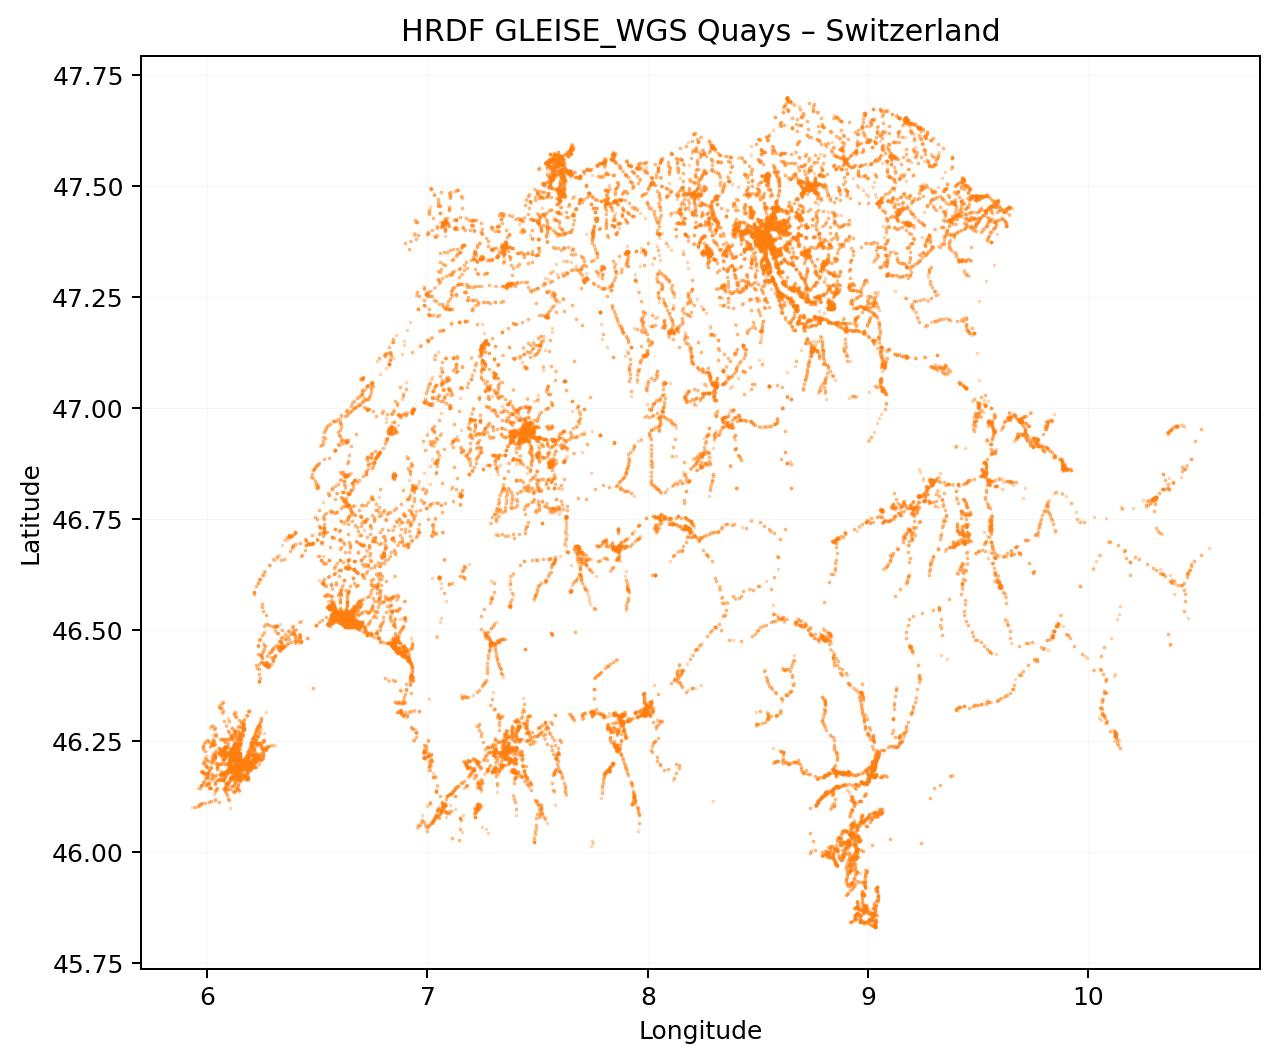
\includegraphics[width=.76\linewidth]{figures/plots/hrdf_quays_switzerland.png}
  \caption[Quais HRDF – Suisse]{Quais HRDF (\texttt{GLEISE\_WGS}) – Suisse.}
\end{figure}


\section{Comparaison GTFS et HRDF (couverture SLOID)}

% 1-plot figure: ATLAS Genève (quais)
\begin{figure}[H]
  \centering
  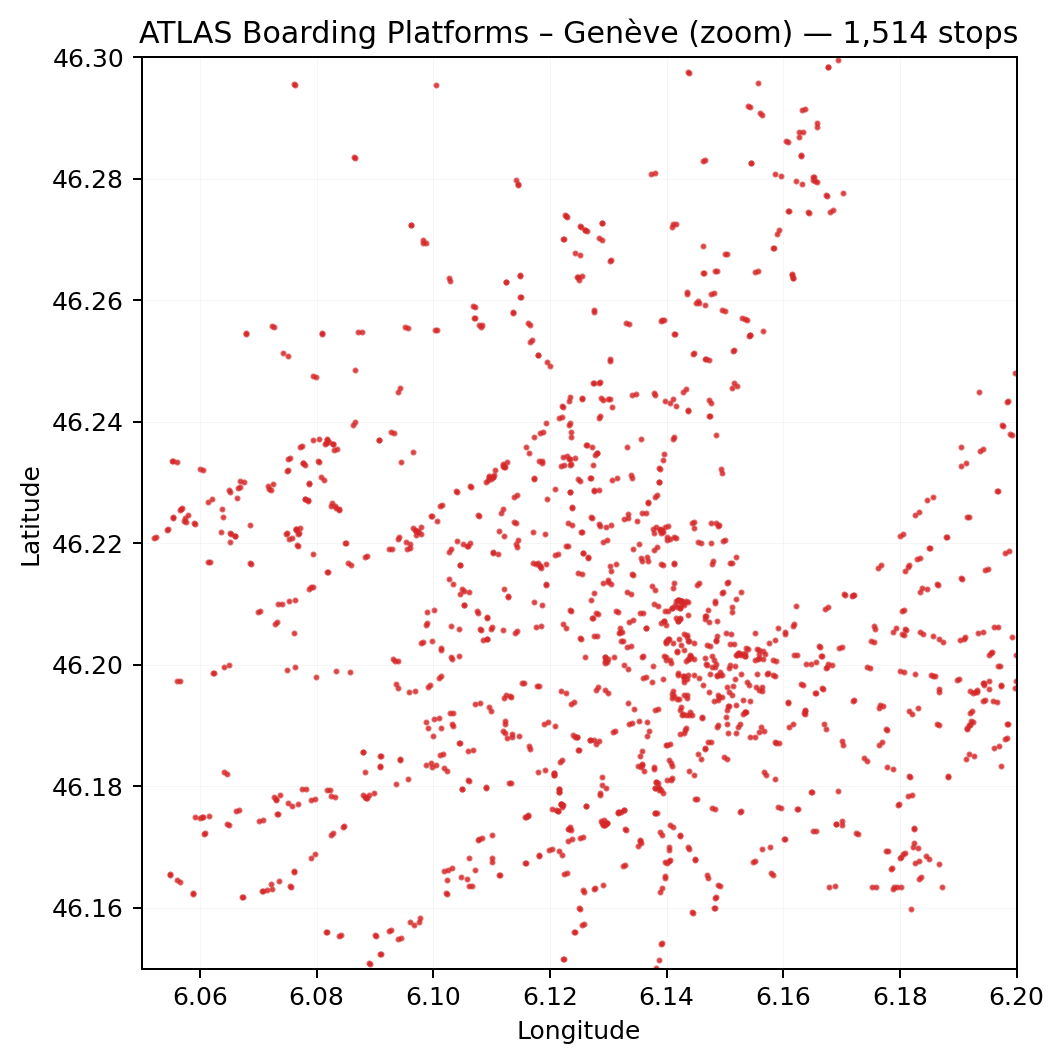
\includegraphics[width=.7\linewidth]{figures/plots/atlas_points_geneva.png}
  \caption[ATLAS – Genève]{ATLAS – plateformes d'embarquement, zoom Genève.}
  \label{fig:atlas_geneva}
\end{figure}

% 2-plot figure: GTFS vs HRDF (points bruts) – Genève
\begin{figure}[H]
  \centering
  \begin{minipage}[t]{0.49\linewidth}
    \centering
    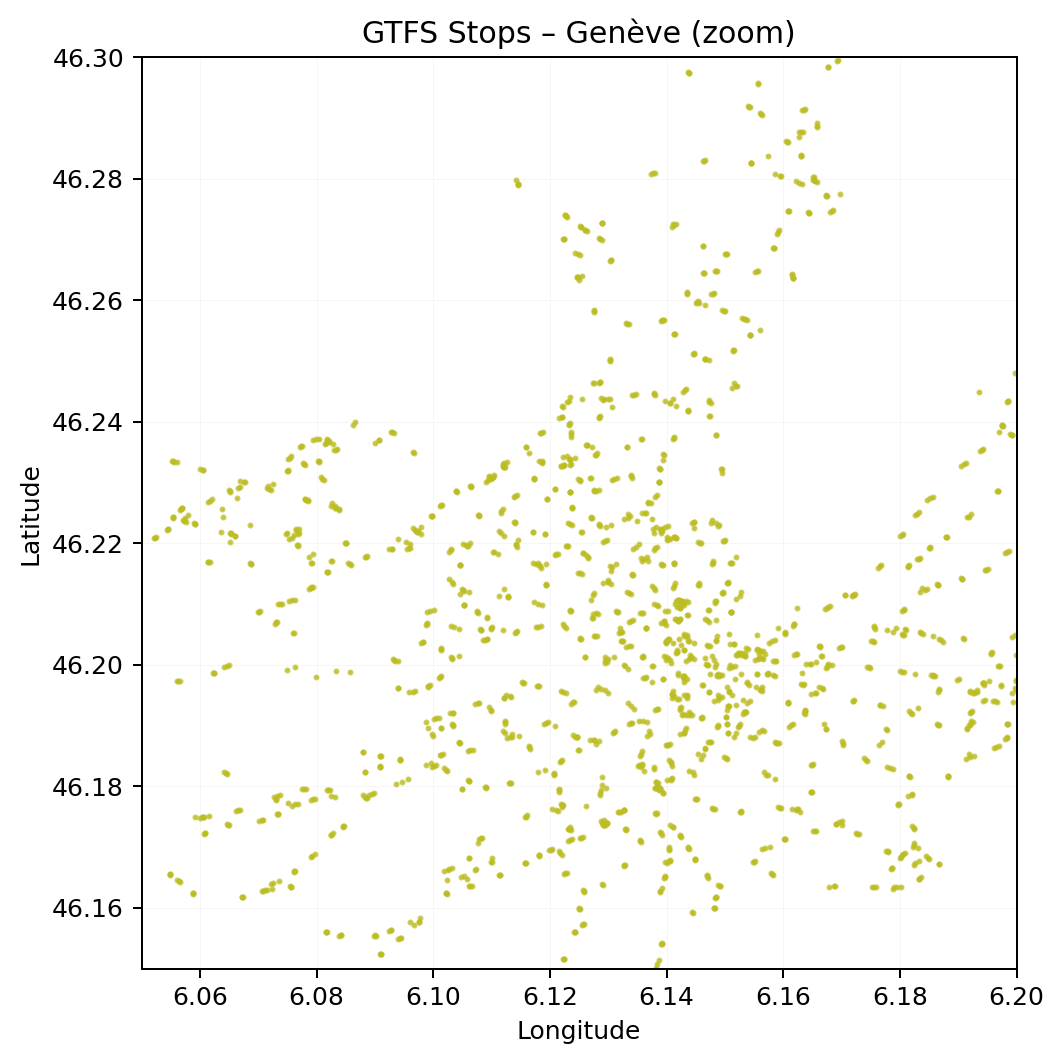
\includegraphics[width=\linewidth]{figures/plots/gtfs_points_geneva.png}
    \vspace{0.2em}
    \small GTFS – arrêts (zoom Genève)
  \end{minipage}\hfill
  \begin{minipage}[t]{0.49\linewidth}
    \centering
    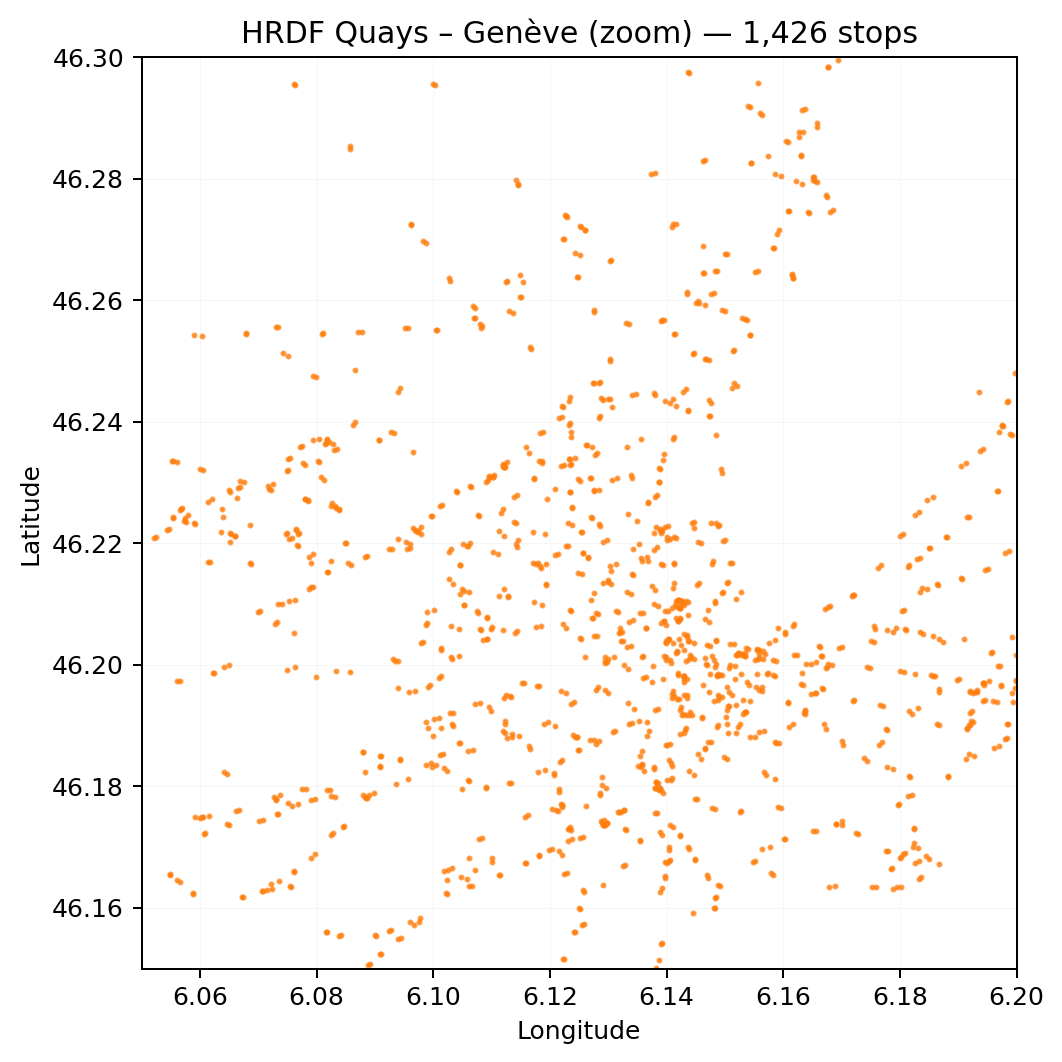
\includegraphics[width=\linewidth]{figures/plots/hrdf_quays_geneva.png}
    \vspace{0.2em}
    \small HRDF – quais (zoom Genève)
  \end{minipage}
  \caption[Genève: GTFS vs HRDF (points bruts)]{Genève: comparaison des points bruts \textbf{GTFS} (gauche) et \textbf{HRDF} (droite).}
  \label{fig:geneva_gtfs_hrdf_raw}
\end{figure}

% 2-plot figure: SLOIDs appariés (GTFS vs HRDF) – Genève
\begin{figure}[H]
  \centering
  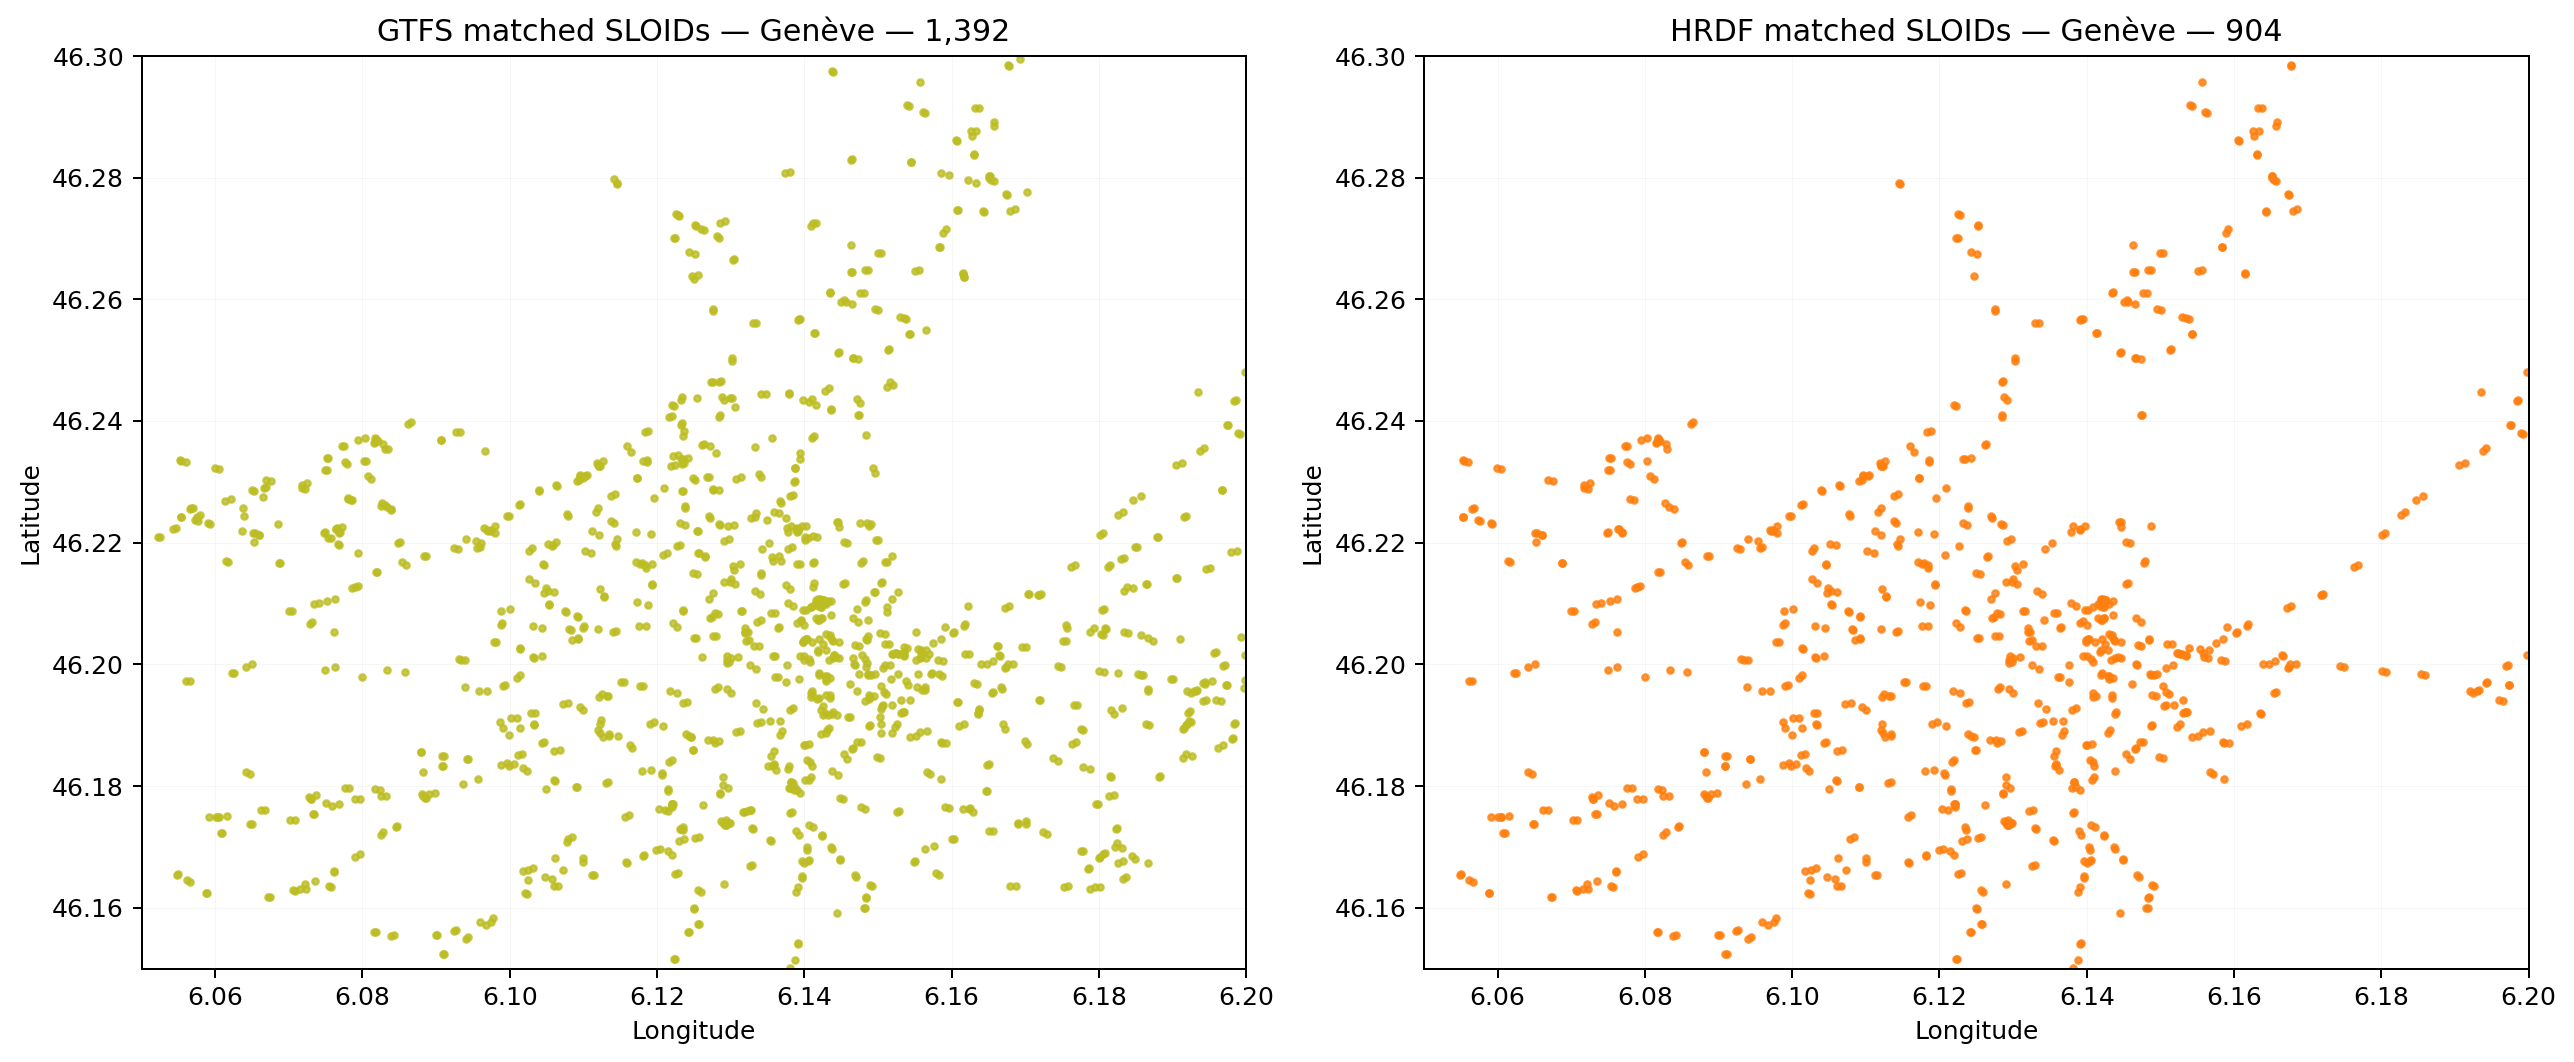
\includegraphics[width=.95\linewidth]{figures/plots/geneva_matched_sloids_gtfs_hrdf.png}
  \caption[Genève: SLOIDs appariés (GTFS vs HRDF)]{Genève: SLOIDs ATLAS couverts par les jeux intégrés \textbf{GTFS} (gauche) et \textbf{HRDF} (droite).}
  \label{fig:geneva_matched_sloids}
\end{figure}

Concernant la couverture globale des SLOIDs ATLAS par les deux jeux de données intégrés, nous observons les statistiques suivantes :

\begin{itemize}
  \item GTFS: \textit{\(34\,415\)} SLOIDs\,; HRDF: \textit{\(28\,723\)} SLOIDs.
  \item Intersection: \textit{\(14\,224\)}\,; GTFS seulement: \textit{\(20\,191\)}\,; HRDF seulement: \textit{\(14\,499\)}.
\end{itemize}